\section{Evaluation on Different Analysis Tasks} \label{sec:analysis-tasks}

\begin{table}[b]
  \centering
  % \begin{tabular}{p{0.08\textwidth}p{0.25\textwidth}p{0.12\textwidth}}
	\begin{tabular}{l l l}
  \toprule
  Name & Type & Data type \\
  \midrule
  boiler & combustion simulation& float64\\
  plasma & magnetic reconnection simulation& float32\\
  diffusivity & hydrodynamics simulation& float64\\
  pressure & hydrodynamics simulation& float64\\
	turbulence & fluid dynamics simulation& float32\\
	kingsnake & CT scan & uint8\\
	foam & CT scan & uint16\\
  \bottomrule
  \end{tabular}\label{tbl:data-sets}
  \vspace{-0.5em}
   \caption{Data sets used in our experiments; all volumes are $64^3$. Additional data sets are 
   included in the supplementary materials}
\end{table}

Thus far, we have presented several types of streams: data-independent (\slvl, \sbit, \swav),
data-dependent and task-independent (\smag), and task-dependent (\sopt, \ssig). In this section, we
consider a variety of common analysis and visualization tasks to evaluate the performance of these
streams. For each task, we define an error metric, $\err$, for the evaluation and comparison of
streams. Using \Cref{alg:greedy}, we compute streams specifically optimized for each task, \stkop,
and use its signature to compute the corresponding \stksg. We compare these streams by evaluating
the error as a function of the number of packets received for a variety of datasets (see
\Cref{tbl:data-sets}). To mimic the effects of compression commonly used in practice, we remove from
each stream all packets that consist only of leading-zero bits. The wavelet basis allows us to
always reconstruct data at full resolution, which greatly simplifies computation of errors, as there
exists no standard method to compute error between grids of different dimensions.

\subsection{Function Reconstruction}\label{sec:rmse-optimized}

\begin{figure*}[t]
\centering
 \subcaptionbox{\label{fig:rmse:boiler}\emph{boiler}}{{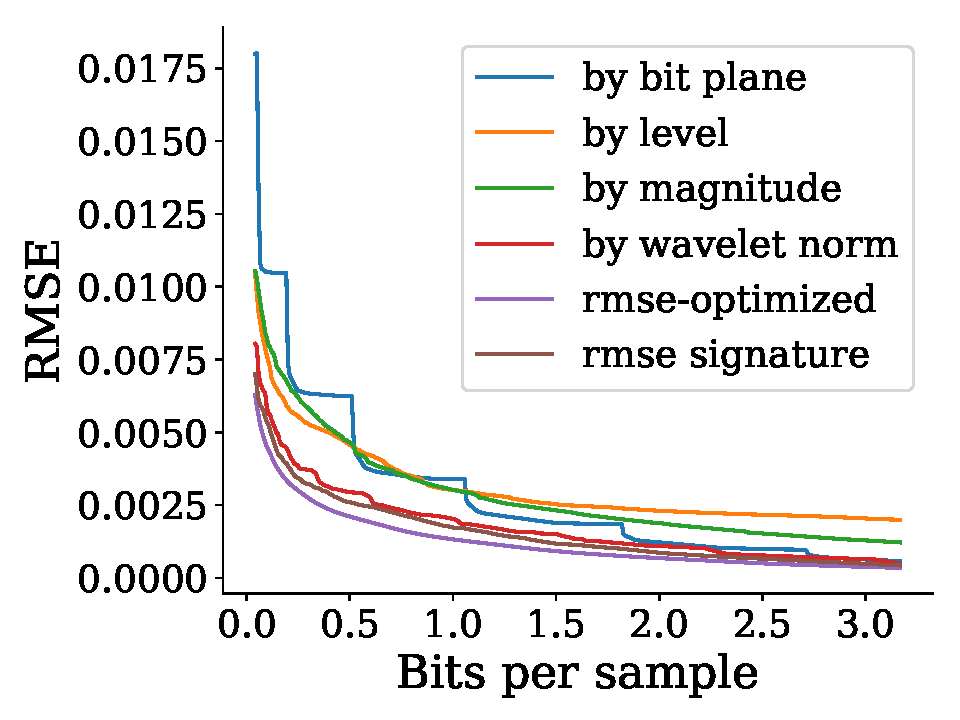
\includegraphics[width=0.24\linewidth]{rmse/rmse-optimized-boiler}}}
 \subcaptionbox{\label{fig:rmse:diffisivity}\emph{diffusivity}}{{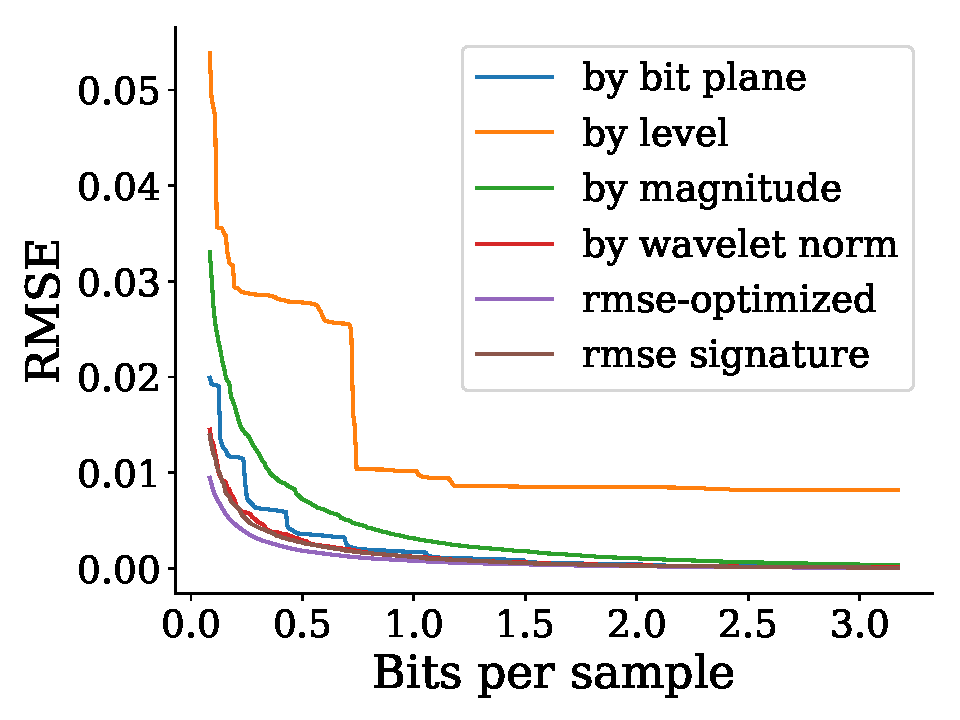
\includegraphics[width=0.24\linewidth]{rmse/rmse-optimized-diffusivity}}}
 \subcaptionbox{\label{fig:rmse:plasma}\emph{plasma}}{ {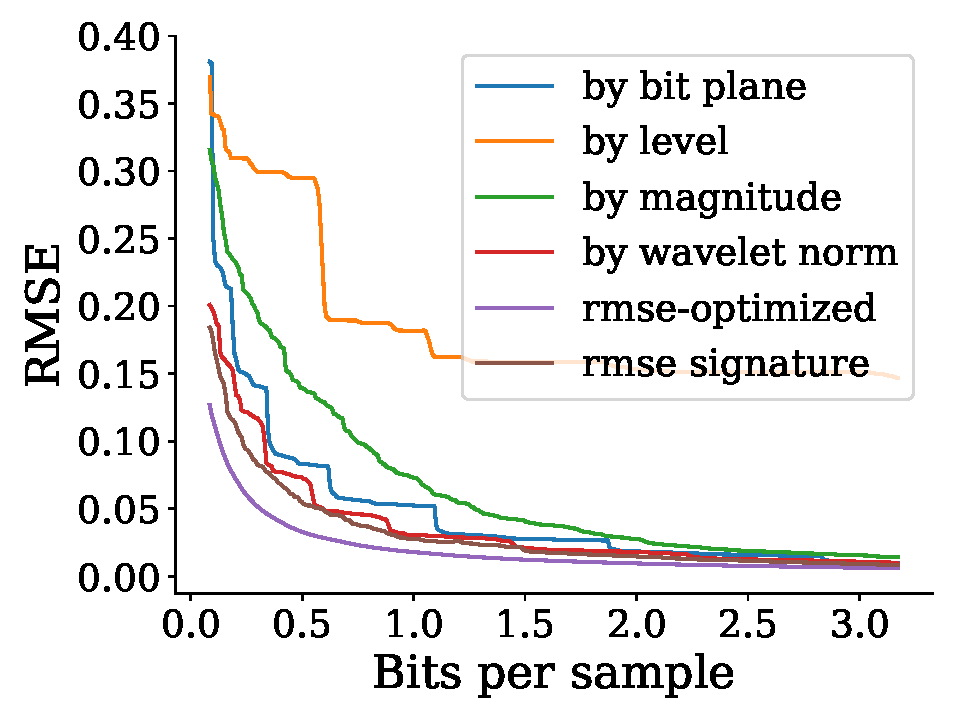
\includegraphics[width=0.24\linewidth]{rmse/rmse-optimized-plasma}}}
 \subcaptionbox{\label{fig:rmse:kingsnake}\emph{kingsnake}}{{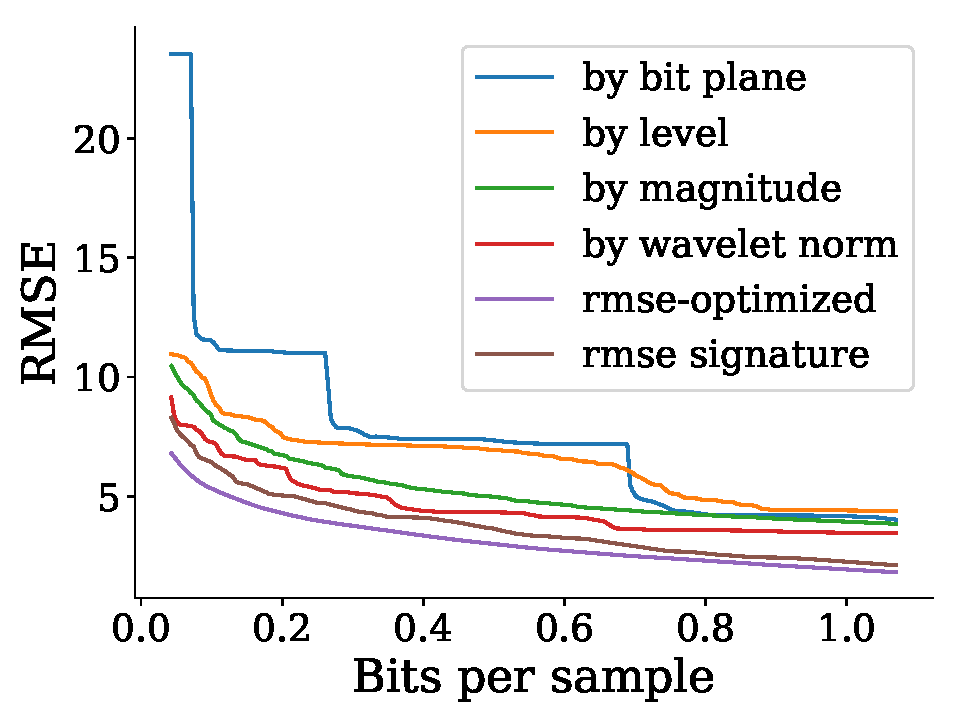
\includegraphics[width=0.24\linewidth]{rmse/rmse-optimized-kingsnake}}}
\caption{Root-mean-square error (RMSE) of reconstructed functions for different streams and data
sets; lower RMSE is better. The streams are truncated at both ends to highlight the differences,
without omitting important information. The general ordering of error, from lowest to highest, is
$\sopt < \ssig < \swav < \sbit < \smag < \slvl$ (for \emph{boiler} and \emph{kingsnake}, \sbit
underperforms \slvl at first, but surpasses its after a certain bit rate).}
\label{fig:rmse-optimized}
\vspace{1em}

\centering
 \subcaptionbox{\emph{by level} (\slvl)}{{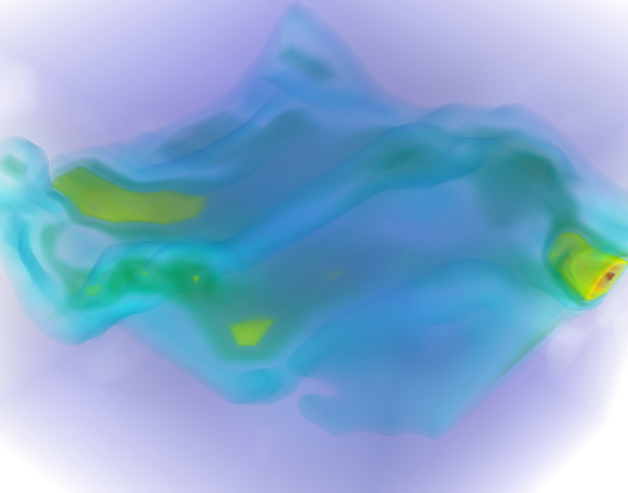
\includegraphics[width=0.16\linewidth]{rmse/rmse-plasma-level}}}
 \subcaptionbox{\emph{by bit plane (\sbit)}}{{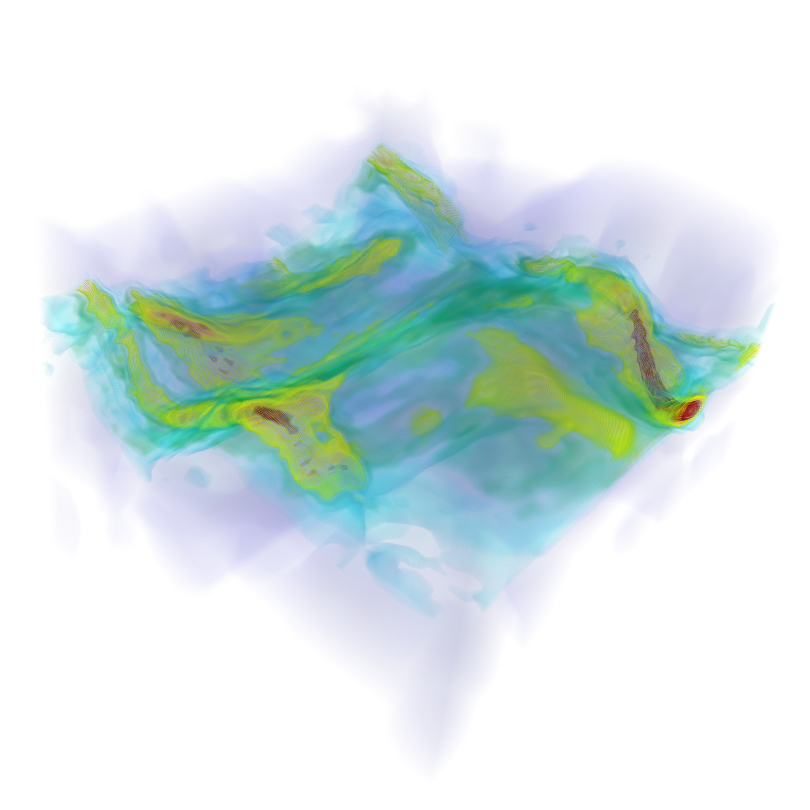
\includegraphics[width=0.16\linewidth]{rmse/rmse-plasma-bit-plane}}}
 \subcaptionbox{\emph{by wavelet norm (\swav)}}{{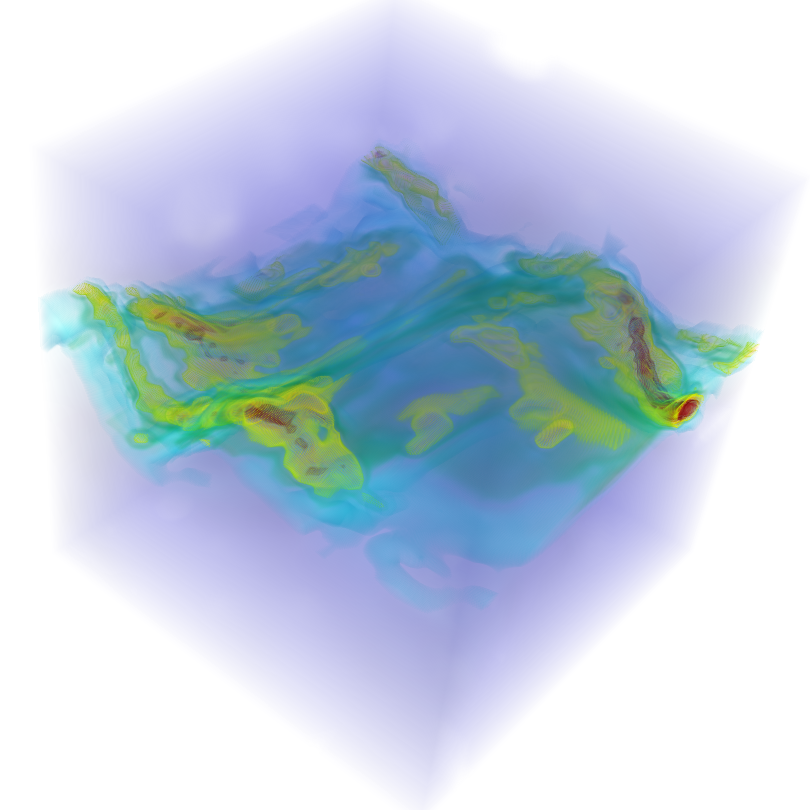
\includegraphics[width=0.16\linewidth]{rmse/rmse-plasma-wavelet-norm}}}
 \subcaptionbox{\emph{by magnitude (\smag)}}{{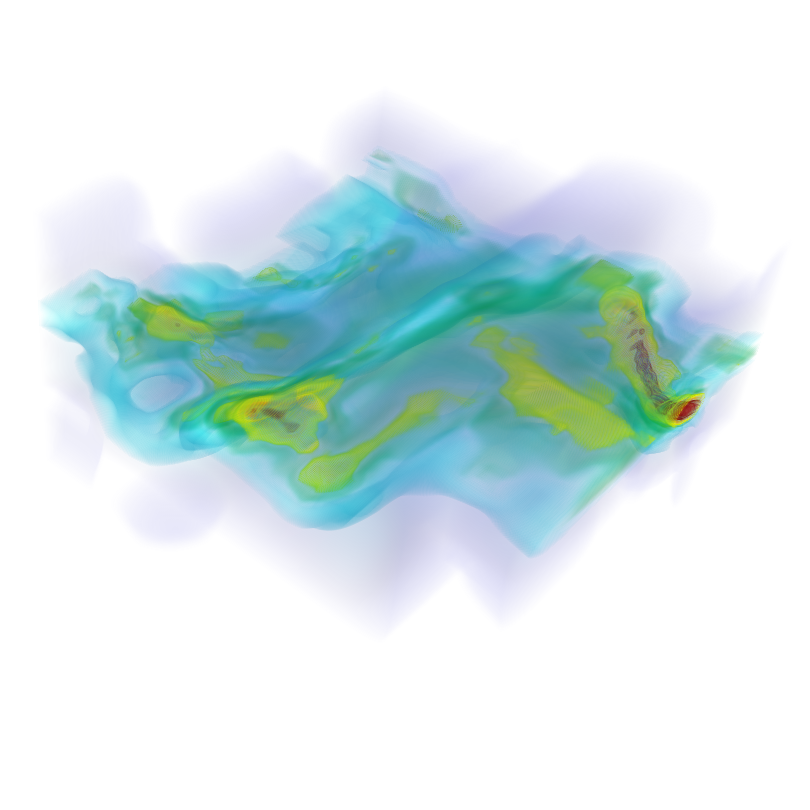
\includegraphics[width=0.16\linewidth]{rmse/rmse-plasma-magnitude}}}
 \subcaptionbox{\emph{by signature (\ssig)}}{{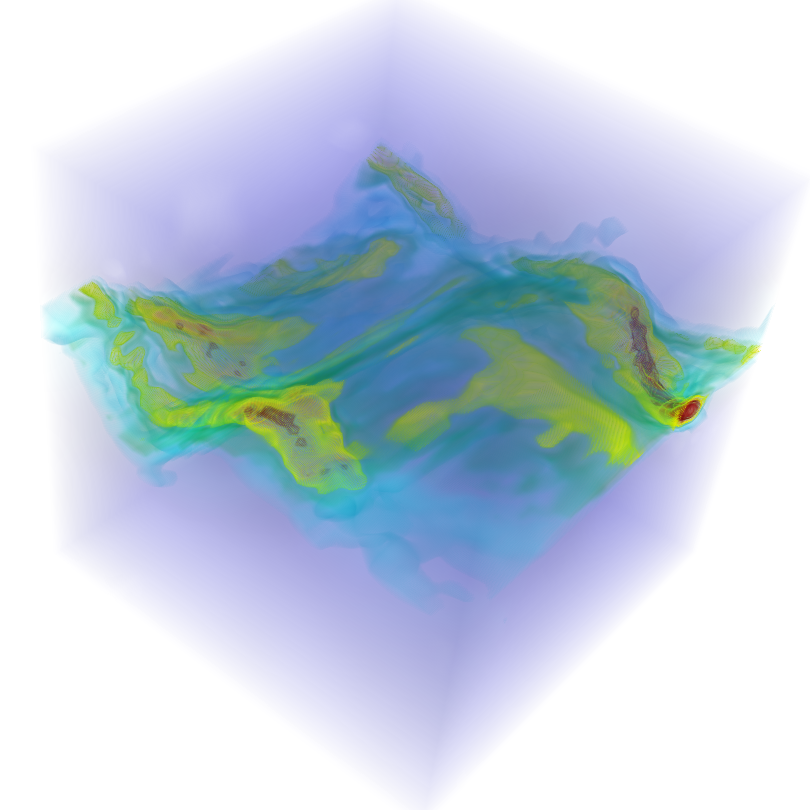
\includegraphics[width=0.16\linewidth]{rmse/rmse-plasma-signature}}}
 \subcaptionbox{\emph{ground truth}}{{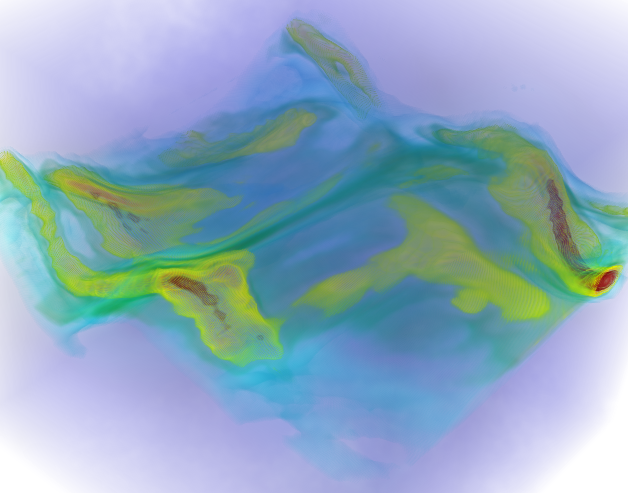
\includegraphics[width=0.16\linewidth]{rmse/rmse-plasma-groundtruth}}}
\caption{Volume renderings of a $64^3$ region of \emph{plasma} data set at 0.1 bps.  \slvl captures
the background (purple-blue) well, whereas \sbit captures the fine details better. \swav combines
the strength of both. \ssig, however, produces the most accurate rendering (compare, e.g., yellow
features).}
\label{fig:rmse-rendering}
\end{figure*}

One of the most fundamental analysis tasks is that of reconstructing the original function itself. A
commonly used error metric in this case is the root-mean-square error
(RMSE).~\Cref{fig:rmse-optimized} shows a comparison of the different streams for a variety of
datasets. It can be noted that, in general, \srop (the stream optimized to minimize the RMSE)
performs better than \srsg due to spatial adaptivity, whereas \srsg slightly outperforms \swav,
followed by \sbit, \smag, and \slvl.

In particular, \sbit outperforms \slvl (for \emph{kingsnake} and \emph{boiler}, it does so after
approximately 1 bps), which can be attributed to the removal of leading-zero packets. Empirically,
wavelet coefficients on finer scale subbands are much smaller in magnitude~\cite{spiht1996}. Such
coefficients contain a majority of the leading-zero bits, whose removal benefits \sbit the most.
\emph{diffusivity} and \emph{plasma} contain a significant amount of empty space, which translates
to more leading-zero bits after the wavelet transform that \sbit can take advantage of. This is the
reason why, unlike for \emph{boiler} and \emph{kingsnake}, \sbit outperforms \slvl immediately from
the beginning for \emph{diffusivity} and \emph{plasma}.

\smag underperforms for the same reason that \slvl does, but to a lesser extent, since \smag is
better adapted to the data. \swav outperforms both \slvl and \sbit, because it follows the optimal
(data-independent) bit ordering in $\Sigma_{L,B}$ in the $L_2$ norm, which is also the norm that
RMSE is based upon. Unsurprisingly, \srop outperforms all the others, as it is the most
data-adaptive (i.e., it can prioritize packets in the spatial domain in addition to the
$\Sigma_{L,B}$ domain). \srsg is the second best stream, as it follows the bit ordering of \srop in
$\Sigma_{L,B}$, but lacks any spatial adaptivity. In general, \swav and \ssig have similar
performance. In some cases (e.g., ~\Cref{fig:rmse:diffisivity} and~\Cref{fig:rmse:plasma}), \ssig is
able to adapt more to the data, thus outperforming \swav by a larger margin.

We explore the errors visually by rendering the \emph{plasma} volume at 0.1 bits per sample (bps), 
for all streams except \srop ~(\Cref{fig:rmse-rendering}). Bps are calculated by dividing
the total size of received packets (in bits) by the total number of samples.
Although \slvl has the precision to obtain an accurate
background, it lacks resolution to resolve the fine details. \sbit, instead, lacks the precision to
reconstruct the (mostly smooth) background, but has enough resolution to capture the fine details
well. \swav balances both precision and resolution, producing a more accurate picture as a whole. In
this case, the \ssig stream manages to produce the most accurate rendering. In general, \srsg
benefits more from ``anisotropic'' data, such as \emph{plasma}, where most features lie on a thin
``surface''. For such data, wavelet coefficients along one dimension are often larger compared to
those along other dimensions, which \srop, and hence \srsg, can take advantage of, but not \swav.
